\documentclass[12pt]{article}
\usepackage[margin=0.3in,top=0.25in,bottom=0.4in]{geometry}
\makeatletter
\renewcommand{\@maketitle}{\newpage\null\vskip -3.5em\begin{center}{\LARGE \@title \par}\end{center}\par\vskip 0.2em}
\makeatother
\usepackage{amsmath,amssymb}
\usepackage{booktabs}
\usepackage{graphicx}
\usepackage{hyperref}
\setlength{\parskip}{0.6em}
\setlength{\parindent}{0pt}
\newcommand{\xpo}{x_{\mathbb{P}}}

\title{Validity of the correlation limit}
\author{}
\date{}

\begin{document}
\sloppy
\maketitle

\section*{In short}

The diffractive TMD factorization holds in the correlation limit, where the hard scale of the
process is much larger than the saturation scale of the target. Figure~\ref{fig:corr} compares the
two for a charm quark at fixed $q^+=2p^+$ ($z=\tfrac12$), proton and Pb at $b_d=0$, $y=0$ to 3 (the range of the bin plots):
\begin{itemize}
\item Gluon DTMD: the hard scale is $M_h=2m_T\geq3$~GeV. For the proton $M_h/Q_{s,A}\gtrsim2.1$ at all
  $p_\perp$. For Pb $M_h/Q_{s,A}\approx1.2$--2 at $p_\perp\lesssim1$~GeV and $\gtrsim3$ only from
  $p_\perp\approx2$~GeV ($y=0$) to 3~GeV ($y=3$): the charm mass keeps the process hard, but the separation is marginal at
  low $p_\perp$.
\item Quark DTMD: the hard scale is $p_\perp$. It crosses $Q_s$ at $p_\perp\approx0.7$--0.9~GeV (proton) and
  $\approx1.2$--1.6~GeV (Pb), so below a few GeV the correlation limit fails. At $p_\perp=5$~GeV,
  $p_\perp/Q_s\approx7$--9 (proton) and 4--5 (Pb), the lower values at $y=3$. This is consistent with including the quark term only
  for $p_c\geq5$~GeV (\texttt{QUARK\_P\_MIN}), but that threshold was chosen from the stability of the
  quark term under the $K_\perp$ cut (changed by 10--20\% at $p_\perp=5$~GeV,
  \texttt{notes/kt\_cut\_and\_quark\_dtmd.pdf}, Sec.~4), not from a condition on $p_\perp/Q_s$.
\end{itemize}

\begin{figure}[h]
\centering
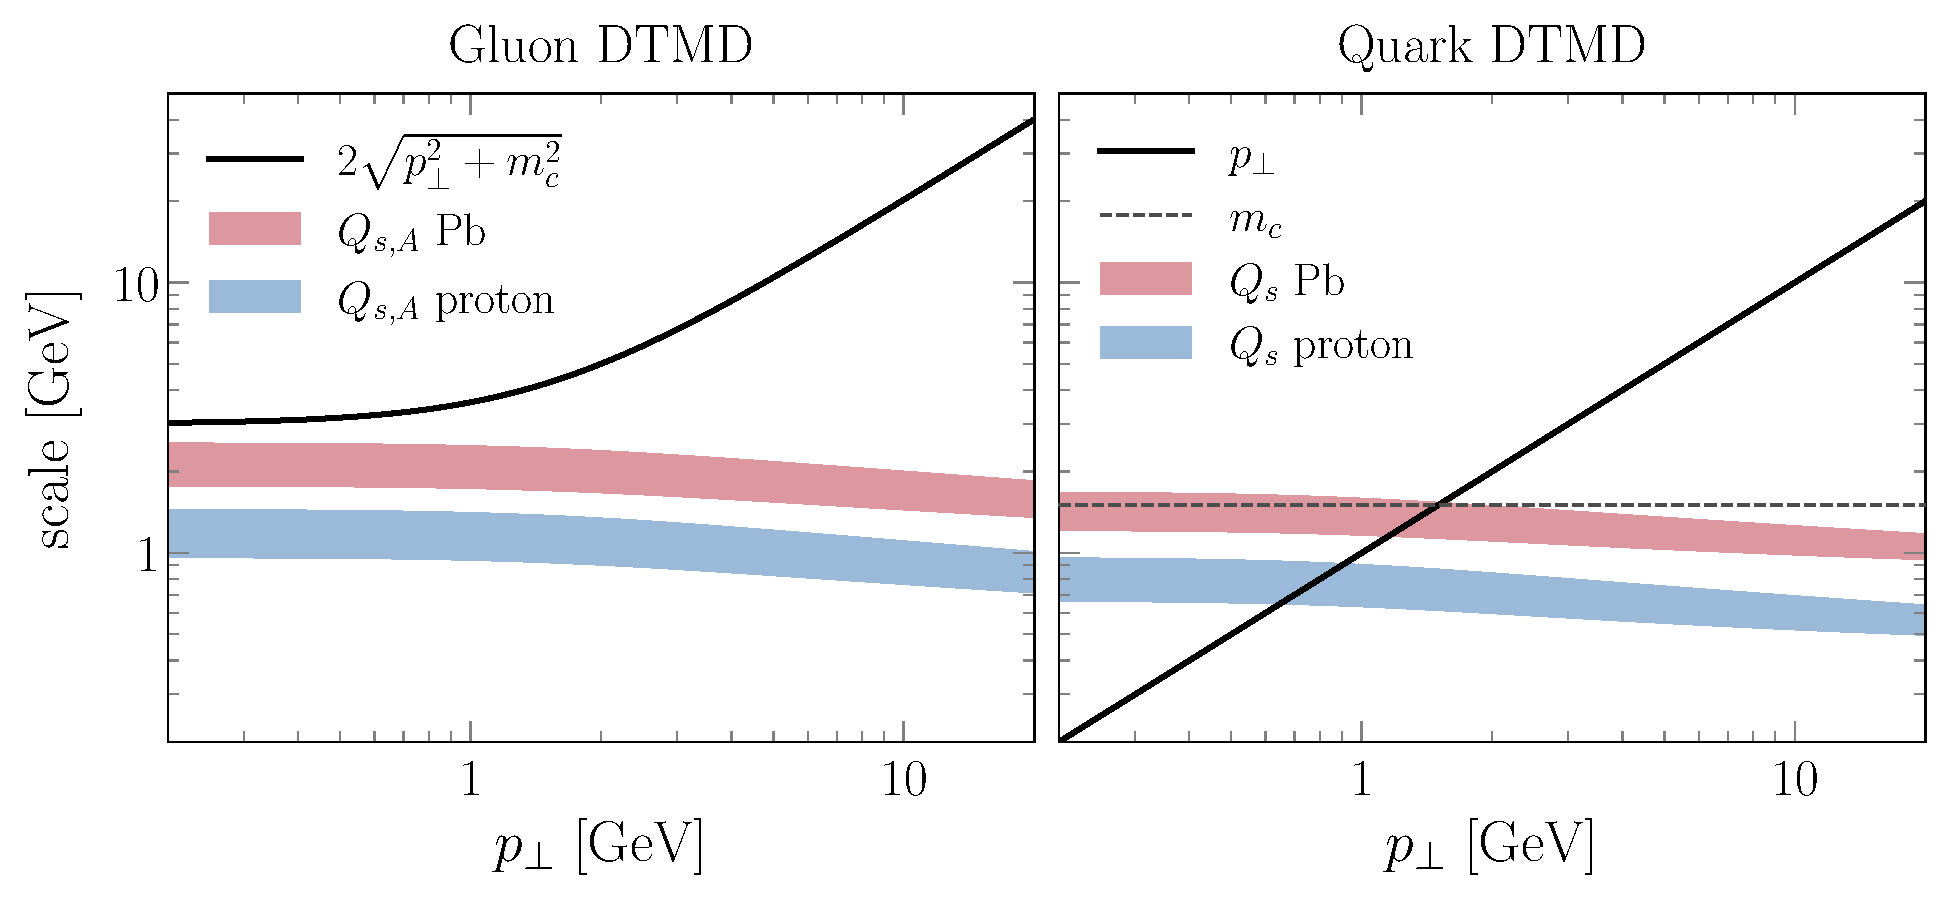
\includegraphics[width=0.95\textwidth]{../plots/correlation_limit.pdf}
\caption{Hard scale (black) against the saturation scale (bands, $y=0$ to 3) for a charm quark at
$q^+=2p^+$. Left: gluon DTMD, $M_h=2m_T$ against the adjoint $Q_{s,A}$. Right: quark DTMD, $p_\perp$
against the fundamental $Q_s$. Pb at $b_d=0$.}
\label{fig:corr}
\end{figure}

\section*{1. Definition of $Q_s$}

The saturation scale is defined from the dipole amplitude at each $x$ as
\begin{equation}
Q_s^2(x)=\frac{2}{r_s^2(x)}\,,\qquad \mathcal{N}(r_s,x)=1-e^{-1/2}\,.
\end{equation}
The fundamental $Q_s$ uses the quark dipole $\mathcal{N}$ (\texttt{AmplitudeLib::SaturationScale}). The
adjoint $Q_{s,A}$ uses the gluon dipole $\mathcal{N}_A=2\mathcal{N}-\mathcal{N}^2=1-(1-\mathcal{N})^2$,
with the same condition $\mathcal{N}_A(r_s)=1-e^{-1/2}$; $r_s$ is found by bisection in $\ln r$.
$\mathcal{N}_A$ comes from the same BK solution: at large $N_c$ a gluon scatters like two quark dipoles.

Each term is compared with the scale of the dipole it contains (\texttt{src/integrands.cpp}):
\begin{itemize}
\item Gluon DTMD: uses $\mathcal{N}_A$. The compact $c\bar c$ pair is a colour octet, so together with
  the soft gluon it scatters like a gluon--gluon dipole $\Rightarrow$ adjoint $Q_{s,A}$.
\item Quark DTMD: uses $\mathcal{N}$. The compact $cg$ pair is a colour triplet, so together with the
  soft antiquark it scatters like a quark--antiquark dipole $\Rightarrow$ fundamental $Q_s$.
\end{itemize}

The value $1-e^{-1/2}$ comes from the GBW form $\mathcal{N}=1-\exp(-r^2Q_s^2/4)$, which at
$r^2=2/Q_s^2$ gives exactly $1-e^{-1/2}$. In GBW,
$\mathcal{N}_A=1-\exp(-r^2Q_s^2/2)$, so $Q_{s,A}^2=2Q_s^2$ and $Q_{s,A}=\sqrt2\,Q_s\approx1.41\,Q_s$.
The BK dipole is less steep in $r$ than GBW, so the ratio is slightly larger: $\approx1.45$--1.5 in the
range of the figure, growing at smaller $x$ (1.7 at $x=10^{-6}$).

The program \texttt{saturation\_scale} (\texttt{src/saturation\_scale.cpp}) writes $Q_s^2$ and
$Q_{s,A}^2$ against $x$ for the proton dipole (\texttt{data/proton/mve.dat}) and for each Pb Glauber file
(\texttt{data/Pb/mve/glauber\_mve\_<b\_d>}), in \texttt{output/saturation\_scale/}
(\texttt{run\_scripts/run\_saturation\_scale.sh}). The figure uses Pb at $b_d=0$, the centre of the
nucleus, where $Q_s$ is largest.

\section*{2. At which $\xpo$}

$Q_s$ grows as $\xpo$ decreases, so we take it at the smallest $\xpo$ each term can reach, which gives
the largest (most conservative) value. The diffractive mass $M^2$ and the photon--target energy fix
\begin{equation}
x=\frac{M^2}{\xpo W^2}<1\quad\Rightarrow\quad \xpo^{\min}=\frac{M^2}{W^2}\,,\qquad
W^2=\sqrt2\,q^+\sqrt{s}=2m_Te^{y}\sqrt{s}\,,
\end{equation}
with $q^+=2p^+=\sqrt2\,m_Te^y$ and $\sqrt{s}=5.36$~TeV. The mass is that of the system produced in each term:
\begin{align}
\text{gluon DTMD } (q\bar q):&\quad M_{q\bar q}^2=\frac{p_\perp^2+m^2}{z\bar z}=4m_T^2\,,\\
\text{quark DTMD } (cg):&\quad M_{cg}^2=\frac{p_\perp^2}{z\bar z}+\frac{m^2}{z}=4p_\perp^2+2m^2\,,
\end{align}
both at $z=\tfrac12$, as in \texttt{src/integrands.cpp}. (The note \texttt{kt\_cut\_and\_quark\_dtmd}
takes instead the smallest $\xpo$ at any photon energy, $z\to0$, which is half as large for the gluon term, so its $Q_s$ are
$\approx10\%$ higher.) Above $\xpo=0.01$ the dipole is frozen at its
initial condition, so $Q_s$ is frozen too. In the range of the figure $\xpo^{\min}$ stays between
$1.4\times10^{-5}$ ($p_\perp=0.2$~GeV, $y=3$) and $7.5\times10^{-3}$ ($p_\perp=20$~GeV, $y=0$), below the
frozen region.

\section*{3. Numbers}

$Q_s$ in GeV at $\xpo^{\min}$, and the ratio of the hard scale to it, for $y=0$ / $y=3$:
\begin{center}
\small
\begin{tabular}{c|cc|cc|cc|cc}
\toprule
 & \multicolumn{4}{c|}{proton} & \multicolumn{4}{c}{Pb, $b_d=0$} \\
$p_\perp$ [GeV] & $Q_{s,A}$ & $M_h/Q_{s,A}$ & $Q_s$ & $p_\perp/Q_s$
 & $Q_{s,A}$ & $M_h/Q_{s,A}$ & $Q_s$ & $p_\perp/Q_s$ \\
\midrule
0.2 & 0.96 / 1.45 & 3.2 / 2.1 & 0.66 / 0.96 & 0.30 / 0.21 & 1.76 / 2.55 & 1.7 / 1.2 & 1.21 / 1.68 & 0.17 / 0.12 \\
0.5 & 0.95 / 1.44 & 3.3 / 2.2 & 0.65 / 0.94 & 0.77 / 0.53 & 1.75 / 2.54 & 1.8 / 1.2 & 1.19 / 1.65 & 0.42 / 0.30 \\
1   & 0.94 / 1.41 & 3.8 / 2.6 & 0.63 / 0.91 & 1.6 / 1.1   & 1.73 / 2.49 & 2.1 / 1.4 & 1.16 / 1.59 & 0.86 / 0.63 \\
2   & 0.90 / 1.35 & 5.6 / 3.7 & 0.60 / 0.84 & 3.4 / 2.4   & 1.67 / 2.39 & 3.0 / 2.1 & 1.10 / 1.50 & 1.8 / 1.3 \\
3   & 0.87 / 1.29 & 7.7 / 5.2 & 0.57 / 0.80 & 5.2 / 3.7   & 1.61 / 2.30 & 4.2 / 2.9 & 1.07 / 1.43 & 2.8 / 2.1 \\
5   & 0.82 / 1.22 & 13 / 8.6  & 0.55 / 0.76 & 9.1 / 6.6   & 1.54 / 2.18 & 6.8 / 4.8 & 1.03 / 1.36 & 4.9 / 3.7 \\
10  & 0.76 / 1.11 & 26 / 18   & 0.52 / 0.70 & 19 / 14     & 1.44 / 2.01 & 14 / 10   & 0.98 / 1.26 & 10 / 7.9 \\
\bottomrule
\end{tabular}
\end{center}
$Q_s$ decreases slowly with $p_\perp$ because $\xpo^{\min}$ grows with the mass; it is larger at $y=3$,
where $\xpo$ is smaller.

\section*{4. Caveats}

\begin{itemize}
\item The definition of $Q_s$ is a convention: another value of $\mathcal{N}(r_s)$, e.g.\ $\tfrac12$
  (\texttt{NS=0.5} in \texttt{run\_saturation\_scale.sh}), shifts the bands. The comparison gives the
  order of magnitude of the separation, not precise thresholds.
\item The bands use $W^2=2m_Te^{y}\sqrt{s}$ for $y=0$ to 3. Rapidities with smaller $W^2$ (e.g.\ the
  negative-$y$ bins of p--Pb in this convention) give a larger $\xpo^{\min}$ and a smaller $Q_s$, so the
  $y=3$ edge is the conservative one.
\item $b_d=0$ is the densest part of the nucleus. The cross section integrates over $b_d$, and at
  larger $b_d$ $Q_s$ is smaller, so the figure is conservative for Pb.
\item $z=p^+/q^+$ is not fixed in the cross section: at fixed $p_\perp$, $y$ of the charm quark it is
  integrated through the photon energy, $q^+$ from $p^+$ to $q^+_{\max}$ ($z$ from 1 down to
  $p^+/q^+_{\max}$, \texttt{photon\_kinematics} in \texttt{src/integrands.cpp}). The figure takes $z=\tfrac12$.
  With $p^+=m_Te^y/\sqrt2$ fixed, $W^2=\sqrt2\,p^+\sqrt{s}/z$ and
  \begin{equation*}
  \text{gluon: } M_h=\frac{m_T}{\sqrt{z\bar z}},\quad \xpo^{\min}=\frac{m_T^2}{\bar z\,\sqrt2\,p^+\sqrt{s}}\,;\qquad
  \text{quark: } \xpo^{\min}=\frac{p_\perp^2/\bar z+m^2}{\sqrt2\,p^+\sqrt{s}}\,.
  \end{equation*}
  For $z>\tfrac12$ both $\xpo^{\min}$ grows ($Q_s$ smaller) and, for the gluon term, $M_h$ grows: the
  condition is easier. For $z<\tfrac12$ (photon energies above $2p^+$) $\xpo^{\min}$ decreases by at most
  a factor 2, so $Q_s$ grows by at most $\approx10\%$ ($Q_s\propto x^{-0.14}$ here). For the gluon term
  this is outweighed by $M_h\propto1/\sqrt{z\bar z}$; for the quark term the hard scale $p_\perp$ does not
  depend on $z$, so $p_\perp/Q_s$ can be up to $\approx10\%$ lower than in the figure.
\end{itemize}

\section*{Files}
Figure: \texttt{plotting\_scripts/correlation\_limit.py} $\to$ \texttt{plots/correlation\_limit.pdf}.
Input: \texttt{output/saturation\_scale/qs\_proton.dat}, \texttt{qs\_Pb\_b0.dat}.

\end{document}
